\section{Wichtige Spezielle Zählprobleme}
Äquivalenzrelationen. Wie viele Äquivalenzrelationen gibt es auf einer $n$-Menge? \\
Dasselbe: Wie viele Partitionen? \\
Einfacher: Wie viele Partitionen in $k ~(\leq n)$ Mengen? \\
\begin{gather*}
	S_{n,k} = S_{n-1,k_1}+ k \cdot S_{n-1,k} \\
	\begin{array}{ c c c c c c c c c }
		n=0	&1	&0	\\
		n=1	&0	&1	&0	\\
		n=2	&0	&1	&1	&0	\\
		n=3	&0	&1	&3	&1	&0	\\
		n=4	&0	&1	&7	&6	&1	&0	\\
		n=5	&0	&1	&15	&25	&10	&1	&0	\\
		n=6	&0	&1	&31	&90	&65	&15	&1	&0	\\
	\end{array} \text{ Sterling-Dreieck 2. Art}\index{Stirling-Dreieck!2. Art}
\end{gather*}

\subsubsection{Permutationen}
Permutation $\pi$ von $n$ Elementen: \\
\begin{gather*}
	\pi : \{ 1, 2, \cdots , n \} \rightarrow \{ 1, 2, \dotsc , n \} \text{ bijektiv} \\
	\begin{pmatrix}
		1		&2		&3		\dots		&n		\\
		\pi(1)		&\pi(2)	&\pi(3)	\dots		&\pi(n)
	\end{pmatrix}
\end{gather*}
\begin{bsp*}
	\begin{gather*}
		\begin{pmatrix}
			1	&2	&3	&4	&5	\\
			5	&4	&3	&2	&1	
		\end{pmatrix} \\
		1 \mapsto 5 \mapsto 1 \\
		2 \mapsto 4 \mapsto 2 \\
		3 \mapsto 3 \\
		\pi \text{ ist \textbf{selbstinvers, Involution}}
	\end{gather*}
\end{bsp*}

\subsubsection{Komposition:}
\begin{gather*}
	\begin{split}
		\begin{pmatrix}
			1	&2	&3	&4	&5	\\
			2	&4	&5	&3	&1	
		\end{pmatrix} \circ \begin{pmatrix}
			1	&2	&3	&4	&5	\\
			5	&1	&2	&4	&3
		\end{pmatrix} = \begin{pmatrix}
			1	&2	&3	&4	&5	\\
			1	&4	&3	&2	&5
		\end{pmatrix} \neq \\
		\neq \begin{pmatrix}
			1	&2	&3	&4	&5	\\
			1	&2	&4	&3	&5	
		\end{pmatrix} = \begin{pmatrix}
			1	&2	&3	&4	&5	\\
			5	&1	&2	&4	&3
		\end{pmatrix} \circ \begin{pmatrix}
			1	&2	&3	&4	&5	\\
			2	&4	&5	&3	&1	
		\end{pmatrix}
	\end{split} \\
	invpi = \begin{pmatrix}	 \todo{Add upsidedown pi with left harpoon leg}
		1	&2	&3	&4	&5	\\
		1	&2	&3	&4	&5
	\end{pmatrix} \text{ Identität } \pi \cdot invpi = \pi \\
	\pi = \begin{pmatrix}
			1	&2	&3	&4	&5	\\
			3	&1	&4	&5	&2	
	\end{pmatrix} \\
	\pi^{-1} = \begin{pmatrix}
			1	&2	&3	&4	&5	\\
			2	&5	&1	&3	&4	
	\end{pmatrix}
\end{gather*}

Regeln:
\begin{itemize}
	\item $\forall \pi_1 , \pi_2 , \pi_3 : ( \pi_1 \circ \pi_2 ) \circ \pi_3 = \pi_1 \circ ( \pi_2 \circ \pi_3 )$
	\item $\exists invpi \forall \pi : \pi \circ invpi = invpi \circ \pi = \pi$ Neutralelement
	\item $\forall \pi \exists \pi^{-1} : \pi \circ \pi^{-1} = \pi^{-1} \circ \pi = invpi$ Inverses
\end{itemize}
$\rightarrow$ Gruppe

Struktur einer Permutation?
\[
	\begin{pmatrix}
		1	&2	&3	&4	&5	&6	&7	&8	&9	&10	\\
		5	&9	&8	&10	&7	&6	&1	&3	&4	&2	
	\end{pmatrix}
\]
Jede Permutation lässt sich \textbf{eindeutig} (bis auf die Reihenfolge der Zyklen) in \textbf{disjunktive Zyklen} zerlegen.
\begin{gather*}
	(6) \circ \underbrace{(3,8)}_{=(8,3)} \circ \underbrace{(1,5,7)}_{\substack{=(7,1,5)\\=(5,7,1)}} \circ (2,9,4,10) \\
	\pi = \begin{pmatrix}
		1	&2	&3	&4	&5	&6	&7	&8	&9	&10	\\
		10	&3	&6	&1	&4	&7	&2	&8	&5	&9	
	\end{pmatrix}\\
	\pi = (8)(1,9,4,10,5)(2,3,6,7) \\
	\pi^{20} = invpi \\
	\pi^2 = (8)(1,9,4,10,5)(2,6)(3,7)
\end{gather*}
Zählen: $S_{n,k} = $ \# Permutationen von $n$ Elementen mit genau $k$ Zyklen.
\begin{gather*}
	S_{0,0} \coloneqq 1 \\
	S_{n,0} = 0 \:(n \geq 1) \\
	S_{n,k} = 0 \:(k > n) \\
	S_{n,n} = 1 (invpi)
	\intertext{Rekursiongleichung}
	S_{n,k} = S_{n-1,k-1} + (n-1) S_{n-1,k}
\end{gather*}

\subsubsection{Stirling-Dreieck 1. Art}\index{Stirling-Dreieck!1. Art}
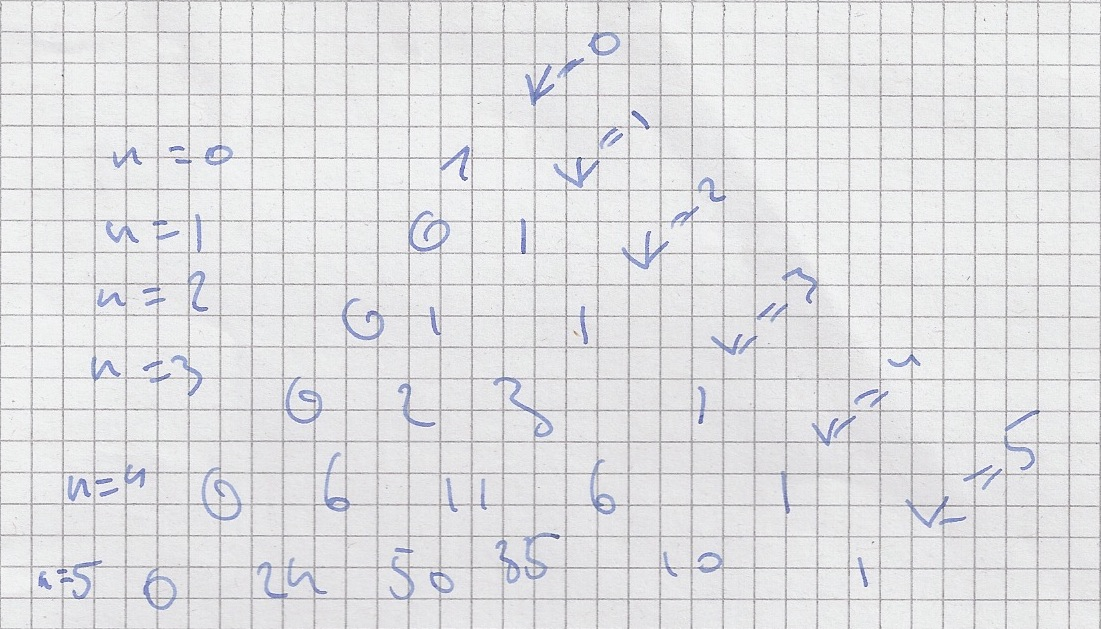
\includegraphics{Bild25}

\subsubsection{Partition von Zahlen}
Auf wie viele Arten kann eine Zahl $n \in \mathbb{N}$ als Summe $n = n_1 + n_2 + \dots + n_k$ von \textbf{positiven} ganzen Zahlen. Wir unterscheiden geordnet / ungeortdnet.
\begin{gather*}
	4 = \left\{ \begin{matrix}
		1	&+	&3	\\
		2	&+	&2	\\
		3	&+	&1	
	\end{matrix} \right. \qquad 4= \left\{ \begin{matrix}
		1	&+	&3	\\
		2	&+	&2	
	\end{matrix} \right.
	\intertext{Ungeordnet:}
	P_{n,k} \\
	\begin{matrix}
		k > n :	& P_{n,k} = 0 \\
		n \geq 1 :	& P_{n,0} = 0 \\
				& P_{0,0} \coloneqq 1 \\
				& P_{n,n} = 1 \\
				& P_{n,1} = 1
	\end{matrix} \\
	\intertext{Rekursion?}
	n > k : n \text{ mit } k \text{ Summanden } \rightarrow n-k \text{ mit } k-i \text{ Summanden } (0 \leq i \leq k-1) \\
	P_{n,k} = \sum_{i=1}^k P_{n-k,i}
	\intertext{Geordnet}
	n = \overbrace{\underbrace{1+1+1}_{n_1} \oplus \underbrace{1+\dots}_{n_2} \oplus \dots \oplus \underbrace{+1}_{n_k}}^n \\
	\binom{n-1}{k-1}
\end{gather*}
Anzahl Möglichkeiten, $n$ als Summe positiver Summanden zu schreiben?
\[ \sum_{k=1}^n \binom{n-1}{k-1} = \sum_{k'=1}^{n-1} \binom{n-1}{k'} = 2^{n-1} \qquad \text{Jedes + unabhängig} \]
